\documentclass[11pt]{article}

\usepackage[margin=1in]{geometry}
\usepackage{amsmath,amssymb,amsthm,mathtools}
\usepackage{booktabs}
\usepackage{lmodern}
\usepackage{microtype}
\usepackage{graphicx}
\usepackage{tikz}
\usetikzlibrary{positioning,arrows.meta}
\usepackage[numbers,sort&compress]{natbib}
\usepackage[colorlinks=true,linkcolor=blue,citecolor=blue,urlcolor=blue]{hyperref}

\newtheorem{theorem}{Theorem}
\newtheorem{proposition}{Proposition}
\newtheorem{definition}{Definition}
\newtheorem{remark}{Remark}

\newcommand{\R}{\mathbb{R}}
\newcommand{\E}{\mathbb{E}}
\newcommand{\norm}[1]{\left\lVert #1 \right\rVert}
\newcommand{\inner}[2]{\left\langle #1, #2 \right\rangle}
\newcommand{\topk}{\mathrm{TopK}}
\DeclareMathOperator*{\argmin}{arg\,min}

\title{\textbf{HALO: An Attention-Free Language Model\\Architecture Built from Compressed Sensing}}
\author{Andrew M.\thanks{\texttt{andrew.jeremy.m@gmail.com}. Code: \texttt{halo\_prototype.py} in the accompanying repository.}}
\date{July 2026}

\begin{document}
\maketitle

\begin{abstract}
Autoregressive transformers store the entire context uncompressed---the key--value cache \emph{is} the raw signal---and reconstruct a context summary at every decoding step by exhaustive pairwise comparison. Compressed learning teaches that this is unnecessary: when a signal is sparse in a suitable dictionary, inference can be carried out directly on a small number of random linear measurements, and reconstruction can be skipped entirely. We take this principle to its logical conclusion and propose \textbf{HALO} (Holographic Autoregressive Language Operator), a causal language model containing no attention, no softmax over positions, and no KV cache. HALO represents every token as a $k$-sparse code over a wide dictionary, maintains context exclusively as a fixed-size multi-timescale \emph{compressive sketch}---a certified restricted-isometry measurement of the sparse context trajectory---and performs all computation in measurement space: retrieval is matched filtering and holographic unbinding, the only nonlinearity is a Top-$K$ operation that coincides with one step of iterative hard thresholding, and network depth is therefore unrolled sparse inference. All temporal mixing is performed by \emph{fixed} structured-random isometries; only pointwise dictionaries, probes, and readouts are learned. Compressed-sensing theory then supplies what heuristic state-space models lack: a closed-form formula for state size as a function of context horizon and sparsity, and a signal-to-noise guarantee for retrieval. Inference requires $O(1)$ memory per sequence and per-token compute independent of context length. A 1.4M-parameter CPU prototype confirms the theory: sketch retrieval SNR matches the predicted $\sqrt{M/kT}$ law to two decimal places, associative recall---the task attention is presumed necessary for---reaches $94.9\%$ accuracy (chance $12.5\%$), and character-level language modeling trains stably to $0.94$ nats/char against a $2.47$ nats/char bigram baseline.
\end{abstract}

\section{Introduction}

The dominant architecture for language modeling stores and repeatedly re-reads an uncompressed record of its own past. At decoding step $t$, a transformer \citep{vaswani2017attention} holds $O(t \cdot d \cdot L)$ key--value states in memory and computes attention scores against all of them, an $O(t)$ operation per token per layer. Modern serving systems such as vLLM \citep{kwon2023pagedattention} exist in large part to manage this cache: paging it, sharing its prefixes, and scheduling around its growth. The memory object being so carefully managed is, from a signal-processing standpoint, a \emph{raw, uncompressed signal}---every past token, kept exactly, forever.

Compressed sensing \citep{candes2006robust,donoho2006compressed} established that signals sparse in some dictionary can be captured by a number of random linear measurements proportional to their information content rather than their ambient dimension, and \emph{compressed learning} \citep{calderbank2009compressed} sharpened the point that matters here: for inference tasks, the signal never needs to be reconstructed at all. A predictor operating directly on measurements $y = \Phi x$ performs nearly as well as one operating on $x$, provided $\Phi$ satisfies the Restricted Isometry Property (RIP) over the relevant sparse family. Reconstruction---the expensive step---is not merely deferrable; it is unnecessary.

This paper asks: \emph{what does a language model look like if reconstruction is made impossible by construction?} We answer with HALO, an architecture assembled entirely from compressed-sensing primitives, governed by four axioms:

\begin{itemize}
  \item[\textbf{A1}] \textbf{Sparsity.} Every internal representation is a $k$-sparse code over a wide dictionary ($k \ll N$). Language is modeled as a sparse trajectory over discrete concepts.
  \item[\textbf{A2}] \textbf{Measurement, not storage.} Context is never stored as a sequence. It exists only as a fixed-size linear sketch $y = \Phi x$ of the sparse trajectory, with $\Phi$ a restricted isometry.
  \item[\textbf{A3}] \textbf{Learning in measurement space.} All trainable computation consumes sketches. Retrieval is matched filtering and holographic unbinding; inference is thresholding of measurement correlations.
  \item[\textbf{A4}] \textbf{Randomness does the mixing.} All interaction across time is mediated by fixed, structured-random linear operators with provable isometry. Only dictionaries, probes, and readouts are learned.
\end{itemize}

\paragraph{Contributions.}
\begin{enumerate}
  \item \textbf{An attention-free architecture} whose recurrent state is a \emph{certified compressed-sensing measurement} of the context, rather than a heuristically sized dense vector (\S\ref{sec:arch}).
  \item \textbf{Capacity by formula.} The state size required for a target recall horizon follows from RIP sampling bounds: $M_b = O(k\,2^b \log N)$ per dyadic timescale band, giving a provable fidelity/memory trade-off that state-space models set by trial and error (\S\ref{sec:theory}).
  \item \textbf{Depth as sparse inference.} The network's only nonlinearity, Top-$K$, is one step of iterative hard thresholding; a stack of $L$ layers is a learned, unrolled sparse solver in the sense of LISTA \citep{gregor2010learning}, giving a precise account of what depth computes (\S\ref{sec:iht}).
  \item \textbf{A retrieval guarantee.} Matched-filter recall from the sketch succeeds with SNR $\sqrt{M/(k\,T_{\mathrm{eff}})}$, degrading smoothly and predictably with load and lag (\S\ref{sec:snr}); we verify the law empirically to two decimal places (\S\ref{sec:exp}).
  \item \textbf{Constant-memory serving.} No KV cache exists; a sequence's entire state is kilobytes, prefill is a parallel associative scan, and state snapshot/fork is a memcpy---dissolving most of the scheduling problem that attention-based serving engines solve (\S\ref{sec:serving}).
\end{enumerate}

\section{Background and Notation}
\label{sec:background}

Let $\Sigma_k = \{x \in \R^N : \norm{x}_0 \le k\}$ denote the set of $k$-sparse vectors.

\begin{definition}[Restricted Isometry Property \citep{candes2005decoding}]
$\Phi \in \R^{M \times N}$ satisfies RIP of order $r$ with constant $\delta_r \in (0,1)$ if for all $x \in \Sigma_r$,
\begin{equation}
(1-\delta_r)\norm{x}_2^2 \;\le\; \norm{\Phi x}_2^2 \;\le\; (1+\delta_r)\norm{x}_2^2 .
\end{equation}
\end{definition}

Random Gaussian matrices satisfy RIP with high probability when $M \ge C\,\delta^{-2}\, r \log(N/r)$ \citep{baraniuk2008simple}; subsampled Fourier/Hadamard matrices with random signs (fast Johnson--Lindenstrauss transforms, FJLT) achieve comparable guarantees with $O(N \log N)$ apply cost and $O(N)$ storage \citep{ailon2009fast,krahmer2011new}. RIP of order $2r$ preserves pairwise inner products of $r$-sparse vectors up to additive error $\delta_{2r}\norm{u}\norm{v}$, which is the property that makes \emph{learning} in measurement space possible:

\begin{theorem}[Compressed learning, informal; \citealp{calderbank2009compressed}]
\label{thm:cl}
Let $\mathcal{D}$ be a distribution over $\Sigma_k \times \{\pm 1\}$ and let $\Phi$ satisfy RIP of order $2k$ with constant $\delta$. Then the soft-margin SVM trained on measurements $\{(\Phi x_i, \ell_i)\}$ achieves hinge loss within $O(\delta)$ of the best linear classifier trained on the $\{(x_i,\ell_i)\}$ themselves.
\end{theorem}

Reconstruction is thus unnecessary for inference. HALO extends this principle from a single linear classifier to a deep autoregressive model by ensuring that every quantity the model computes is a (learned) function of RIP measurements of sparse signals.

Two further ingredients: \emph{iterative hard thresholding} (IHT), the recursion $a^{(i+1)} = \topk_r\!\big(a^{(i)} + \Phi^\top(y - \Phi a^{(i)})\big)$, converges linearly to the sparse code explaining $y$ whenever $\delta_{3r} < 1/\sqrt{32}$ \citep{blumensath2009iterative}; and \emph{holographic unbinding} from vector-symbolic architectures \citep{plate1995holographic,kanerva2009hyperdimensional}, where correlation (elementwise product in a transform domain) retrieves items from an additive superposition.

\section{The HALO Architecture}
\label{sec:arch}

\subsection{Signal model: language as a sparse trajectory}
\label{sec:signal}

Fix a wide concept dictionary of $N$ atoms with low mutual coherence. At step $t$, token $x_t$ is encoded as a $k$-sparse code $s_t \in \Sigma_k \subset \R^N$ with $k \ll N$. The \emph{context signal} is the decayed, position-bound superposition
\begin{equation}
\label{eq:context}
x_t \;=\; \sum_{j \le t} \lambda^{\,t-j}\, P^{\,t-j} s_j ,
\end{equation}
where $P$ is a fixed random signed permutation of $\R^N$ (a unitary \emph{time-binding} operator in the VSA sense) and $\lambda \in (0,1)$ a decay. Two facts make \eqref{eq:context} compressible. First, each term is $k$-sparse and $P^{\,t-j}$ maps supports to incoherent locations, so the superposition behaves like a concatenation in general position. Second, decay imposes an effective horizon $T_{\mathrm{eff}} = 1/(1-\lambda)$: terms older than $\sim T_{\mathrm{eff}}$ fall below the crosstalk floor. Hence $x_t$ is effectively $(k\,T_{\mathrm{eff}})$-sparse. HALO never forms $x_t$; it maintains only its measurement.

\subsection{Sparse semantic coder}

\begin{equation}
s_t = \topk_k\big(E[x_t]\big), \qquad E \in \R^{V \times N} \text{ learned, rows renormalized},
\end{equation}
where $\topk_k$ retains the $k$ largest entries of $\mathrm{relu}(\cdot)$ (values kept, remainder zeroed); gradients flow through the surviving coordinates. A coherence regularizer (\S\ref{sec:training}) keeps the learned dictionary compatible with the RIP assumptions.

\subsection{The context sketch (replaces the KV cache)}
\label{sec:sketch}

Layer $\ell$ maintains $B$ \emph{bands}, each a measurement vector $y^{(\ell,b)} \in \R^{M_b}$. Per token,
\begin{equation}
\label{eq:sketch}
y_t^{(\ell,b)} \;=\; \lambda_b \,\Pi_b\!\left(y_{t-1}^{(\ell,b)}\right) \;+\; \Phi^{(\ell,b)}\, a_t^{(\ell-1)} ,
\end{equation}
with the following components:
\begin{itemize}
  \item $\Phi^{(\ell,b)} \in \R^{M_b \times N}$: a \emph{fixed} structured-random measurement operator (at scale, an FJLT: apply in $O(N\log N)$, store in $O(N)$);
  \item $\Pi_b$: a fixed random signed permutation of $\R^{M_b}$---the time-binding operator pushed into measurement space (commuting binding into the sketch keeps all state $M$-dimensional);
  \item $\lambda_b$: a scalar decay on a dyadic ladder $\lambda_b = 1 - 2^{-b}$, giving horizons $T_{\mathrm{eff}}(b) = 2^b$, $b = 1,\dots,B$, with band widths $M_b$ set by the capacity formula of \S\ref{sec:capacity}.
\end{itemize}

Equation \eqref{eq:sketch} is a \emph{linear} recurrence: it admits a parallel associative scan at training time (as in S5/Mamba \citep{smith2023s5,gu2023mamba}) and an $O(1)$ sequential update at inference. The entire per-sequence state is $\sum_b M_b$ floats per layer---kilobytes, not gigabytes.

The load-bearing novelty is that this state is not a learned dense RNN vector but a \emph{certified compressed-sensing measurement} of the effectively $(k\,T_{\mathrm{eff}})$-sparse context signal \eqref{eq:context}. Everything CS theory asserts about $y = \Phi x$---capacity, retrievability, SNR---applies verbatim, with constants known in advance.

\subsection{PTR: probe--threshold--recode (replaces attention and the FFN)}
\label{sec:ptr}

Attention answers ``what in the context is relevant now, and what does it imply?'' HALO answers the same question with matched filtering, holographic unbinding, and thresholding---never with pairwise position comparisons:
\begin{align}
z_t &= \sum_b \Big[\, W_q^{(b)}\, y_t^{(\ell,b)} \;+\; W_c^{(b)} \big( \Phi^{(b)} a_t^{(\ell-1)} \odot y_t^{(\ell,b)} \big) \Big] \;+\; W_d\, a_t^{(\ell-1)} , \label{eq:probe}\\
a_t^{(\ell)} &= \topk_k(z_t) \;+\; a_t^{(\ell-1)} . \label{eq:recode}
\end{align}

\paragraph{Probe ($W_q$).} Row $i$ of $W_q^{(b)}$ is a learned filter $q_i \in \R^{M_b}$. Because $\Phi$ is a near-isometry, $\inner{q_i}{y} \approx \inner{\Phi^{+} q_i}{x}$: each probe measures the presence and strength of a learned concept configuration \emph{in the context signal}, at that band's timescale, without reconstructing it. The canonical special case $q_i = \Phi\, \Pi^{j} \psi_v$ is the matched filter for ``concept $v$ occurred $j$ steps ago'' (\S\ref{sec:snr}); learned probes are soft conjunctions of such detectors.

\paragraph{Unbinding ($W_c$).} The additive probe alone cannot perform \emph{content-dependent} lookup---retrieval conditioned on the current token requires a bilinear interaction between query and context. The $W_c$ path supplies it CS-natively: $\Phi a \odot y$ is the coordinatewise correlation of the current code's measurement against the sketch, the holographic unbinding operation of VSAs \citep{plate1995holographic}, executed in measurement space at $O(M_b)$ cost with no per-position comparisons. Ablation confirms this term is what converts associative recall from ${\sim}3.6{\times}$ chance to ${\sim}95\%$ accuracy (\S\ref{sec:recall}).

\paragraph{Threshold.} $\topk_k$ is one step of IHT (\S\ref{sec:iht}); the residual connection in \eqref{eq:recode} keeps supports from collapsing (a union of two $k$-sparse codes is at most $2k$-sparse). There is no softmax anywhere in the network; Top-$K$ is the only nonlinearity---the CS-native one.

\subsection{Readout}

\begin{equation}
\mathrm{logits}_t \;=\; W_o\, a_t^{(L)} \;+\; W_r \big[\, y_t^{(L,1)}; \cdots ; y_t^{(L,B)} \big],
\end{equation}
where the second term gives the output head direct matched-filter taps into the top-layer sketch, useful for copy/recall behavior (routing ``the token bound at lag $j$'' to the logits without spending dictionary capacity on it).

\begin{figure}[t]
\centering
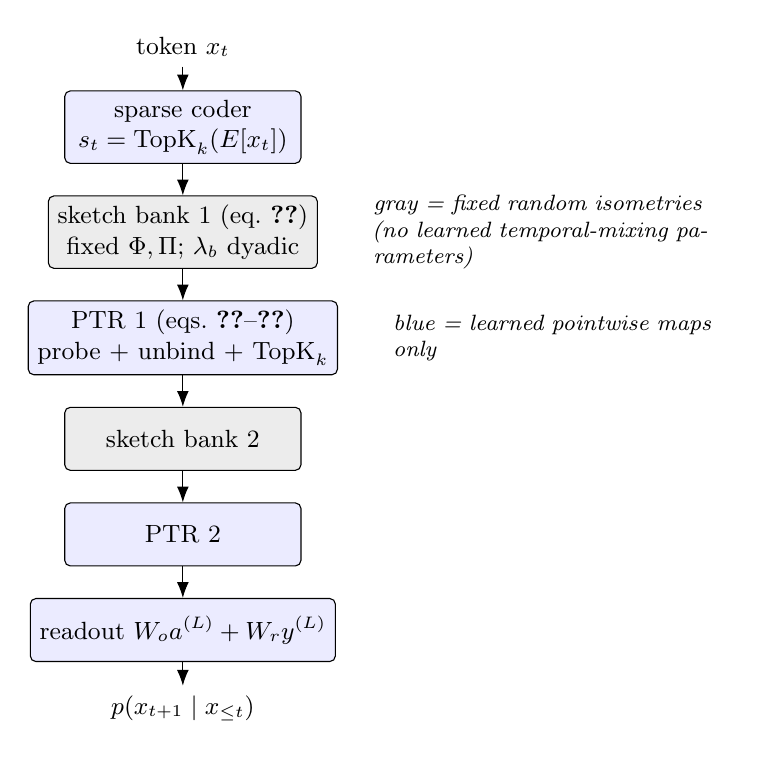
\begin{tikzpicture}[
  node distance=4mm and 8mm,
  box/.style={draw, rounded corners=2pt, minimum height=8mm, minimum width=30mm, align=center, font=\small},
  fixed/.style={box, fill=gray!15},
  learned/.style={box, fill=blue!8},
  arr/.style={-{Latex[length=2mm]}}
]
\node[learned] (emb) {sparse coder\\ $s_t = \topk_k(E[x_t])$};
\node[fixed, below=of emb] (sk1) {sketch bank 1 (eq.~\ref{eq:sketch})\\ fixed $\Phi,\Pi$; $\lambda_b$ dyadic};
\node[learned, below=of sk1] (ptr1) {PTR 1 (eqs.~\ref{eq:probe}--\ref{eq:recode})\\ probe + unbind + $\topk_k$};
\node[fixed, below=of ptr1] (sk2) {sketch bank 2};
\node[learned, below=of sk2] (ptr2) {PTR 2};
\node[learned, below=of ptr2] (ro) {readout $W_o a^{(L)} + W_r y^{(L)}$};
\node[above=3mm of emb, font=\small] (tok) {token $x_t$};
\node[below=3mm of ro, font=\small] (out) {$p(x_{t+1}\mid x_{\le t})$};
\draw[arr] (tok) -- (emb);
\draw[arr] (emb) -- (sk1);
\draw[arr] (sk1) -- (ptr1);
\draw[arr] (ptr1) -- (sk2);
\draw[arr] (sk2) -- (ptr2);
\draw[arr] (ptr2) -- (ro);
\draw[arr] (ro) -- (out);
\node[right=6mm of sk1, font=\footnotesize, align=left, text width=44mm] {\emph{gray = fixed random isometries (no learned temporal-mixing parameters)}};
\node[right=6mm of ptr1, font=\footnotesize, align=left, text width=44mm] {\emph{blue = learned pointwise maps only}};
\end{tikzpicture}
\caption{The HALO stack: alternating fixed-random temporal compression (sketch banks) and learned measurement-domain sparse inference (PTR layers). Context exists only as the sketch state; no sequence of past activations is ever stored.}
\label{fig:arch}
\end{figure}

\subsection{Associative recall without induction heads}
\label{sec:bigram}

The transformer's induction head (locate the previous occurrence of the current token; copy its successor) has a closed-form HALO realization. Layer-1 codes act as coincidence detectors over the fast band: an atom receiving simultaneous input from the sketch (previous token) and the direct path (current token) survives $\topk$ competition, yielding \emph{bigram atoms}. These are superposed into layer-2's sketch. At query time, the unbinding path correlates the current key's measurement against that sketch; stored bigram atoms containing the key light up, $\topk$ selects them, and the readout maps the winning atom to its bound value. One probe, $O(M)$ work, independent of how far back the pair occurred (within the band's horizon).

\section{Theory}
\label{sec:theory}

\subsection{Learning transfer}

By Theorem~\ref{thm:cl} and the inner-product preservation afforded by RIP of order $2r$, any function that a downstream predictor could learn from linear functionals of the context signal $x_t$, HALO's probes can learn from the sketch $y_t$ at an $O(\delta)$ penalty. The nonlinear stack then composes such functionals; each PTR layer re-codes into a new sparse frame to which the argument applies afresh.

\subsection{Sketch capacity: state size by formula}
\label{sec:capacity}

The context signal at band $b$ is effectively $r_b$-sparse with $r_b = k\,T_{\mathrm{eff}}(b) = k\,2^b$. RIP sampling bounds \citep{baraniuk2008simple} then dictate
\begin{equation}
\label{eq:capacity}
M_b \;=\; C\, k\, 2^{b} \,\log\!\big(N / (k 2^b)\big).
\end{equation}
Dyadic bands $b = 1,\dots,B$ cover horizons up to $T = 2^B$ with total per-layer state
\begin{equation}
\sum_b M_b = O\!\big(k\,2^B \log N\big) \quad\text{truncated at horizon } 2^B \text{ with graceful degradation beyond.}
\end{equation}
Where a transformer pays $O(T \cdot d)$ memory to keep every position exactly, HALO chooses a point on a \emph{provable} fidelity/memory curve: ``exact recall to horizon 4096, statistical gist beyond'' becomes a budget line item rather than an emergent accident. This is the design dial that state-space models lack---their state size is a hyperparameter justified post hoc, while $M_b$ is a theorem.

\subsection{Retrieval SNR}
\label{sec:snr}

\begin{proposition}[Matched-filter recall]
\label{prop:snr}
Let $y_t$ be the band sketch of \eqref{eq:sketch} with decay $\lambda$, and let $q = \Phi\,\Pi^{j}\psi_v$ (unit-norm) be the matched filter for atom $v$ at lag $j$. Then
\begin{equation}
\inner{q}{y_t} = \lambda^{j}\alpha_v + \varepsilon, \qquad
\mathrm{SNR} \;\asymp\; \lambda^{j}\,\lvert\alpha_v\rvert\, \sqrt{\frac{M}{k\,T_{\mathrm{eff}}}} ,
\end{equation}
where $\alpha_v$ is the stored coefficient and $\varepsilon$ is crosstalk from the remaining $\sim k\,T_{\mathrm{eff}}$ active atoms, with variance $\norm{x}^2/M$ under random $\Phi$.
\end{proposition}

Detection of a unit-strength atom at lag $j$ therefore succeeds with high probability once $M \gtrsim k\,T_{\mathrm{eff}} \log N \cdot \lambda^{-2j}$, consistent with \eqref{eq:capacity}. Retrieval quality degrades smoothly and predictably with lag and load: the model has a physics, not merely a parameter count. Section~\ref{sec:exp0} verifies the $\sqrt{M/kT}$ law empirically.

\subsection{Depth is unrolled sparse inference}
\label{sec:iht}

A PTR layer computes $a = \topk_k(W_q y + \dots)$. With $W_q = \Phi^\top$ this is exactly one IHT step for the inverse problem ``which sparse code explains this sketch?'', and IHT converges linearly whenever $\delta_{3r} < 1/\sqrt{32}$ \citep{blumensath2009iterative}. Learned $W_q \neq \Phi^\top$ is precisely the LISTA move \citep{gregor2010learning}: learned unrolled iterations converge in far fewer steps than the prescribed operator. A depth-$L$ HALO is thus $L$ steps of accelerated sparse inference over a hierarchy of learned dictionaries---a falsifiable account of what depth computes, which the transformer lacks.

\subsection{Expressivity}

The sketch recurrence \eqref{eq:sketch} is linear, so a single layer computes only functionals of $\sum_j \lambda^{j}\Pi^{j}\Phi s_{t-j}$. But $\topk$ re-codes nonlinearly between layers, and layer $\ell{+}1$ sketches the \emph{nonlinear} stream $a^{(\ell)}$. The alternation (linear temporal mixing $\circ$ pointwise sparse nonlinearity)$^L$ is the same skeleton that underlies the expressivity of deep SSM stacks \citep{gu2022s4,gu2023mamba}; HALO inherits those constructions with binding playing the role of shift/convolution tricks, and adds the bilinear unbinding path, which is strictly necessary for content-conditioned retrieval (\S\ref{sec:recall}).

\section{Complexity and Serving}
\label{sec:serving}

\begin{table}[h]
\centering
\small
\begin{tabular}{llll}
\toprule
\textbf{HALO operation} & \textbf{Cost} & \textbf{Transformer analogue} & \textbf{Cost} \\
\midrule
sketch update \eqref{eq:sketch} & $O(N\log N + \sum_b M_b)$ & KV append + attention & $O(T\,d)$ \\
probe $W_q y$, unbind $W_c(\cdot)$ & $O(N \sum_b M_b)$ dense & $\mathrm{softmax}(QK^\top)V$ & $O(T\,d)$ \\
$\topk_k$ over $N$ & $O(N)$ & FFN & $O(d^2)$ \\
\textbf{sequence state} & $\boldsymbol{\sum_b M_b}$ \textbf{floats (KBs)} & \textbf{KV cache} & $\boldsymbol{O(T\,d\,L)}$ \textbf{(GBs)} \\
\bottomrule
\end{tabular}
\caption{Per-token, per-layer costs. HALO's per-token compute is independent of context length $T$.}
\label{tab:complexity}
\end{table}

The serving consequences are structural. With no KV cache there is no paging, no eviction policy, and no prefix-sharing machinery \citep{kwon2023pagedattention}; a sequence is a fixed-size vector, so continuous batching degenerates to dense matmul batching. Prefill is an associative scan of a linear recurrence ($O(\log T)$ depth, fully parallel). State snapshot and restore---for speculative decoding, beam branching, or agent forking---is a memcpy of kilobytes. The scheduling problem that attention-serving engines exist to solve largely disappears; the engine becomes a streaming dense-batch pipeline.

\section{Training}
\label{sec:training}

\textbf{Objective.} Standard next-token cross-entropy, end-to-end. The scan \eqref{eq:sketch} is linear with spectral radius $\lambda_b < 1$: no exploding modes; vanishing is by design and compensated by slow bands.

\textbf{Top-$K$ gradients.} Exact on surviving coordinates (selection is piecewise constant almost everywhere). Dead-atom collapse is mitigated by a load-balancing penalty $\sum_i (\mathrm{usage}_i - k/N)^2$, as in sparse-MoE routers \citep{fedus2022switch}, and optionally by annealing $k$ downward early in training.

\textbf{Coherence regularization.} $\mathcal{L}_\mu = \norm{\bar E^\top \bar E - I}^2_{F,\mathrm{offdiag}}$ on the (row-normalized) dictionary keeps learned atoms incoherent---this is what keeps the CS guarantees honest for learned dictionaries.

\textbf{Frozen mixing.} $\Phi$ and $\Pi$ are never trained. This removes essentially all temporal-mixing parameters from the optimization: HALO trains only pointwise maps ($E, W_q, W_c, W_d, W_o, W_r$). If needed, $\Phi$ can be fine-tuned late in training with the coherence penalty active.

\textbf{Curriculum.} Context length grows with band count $B$; each new band initializes fresh while earlier bands remain trained, giving cheap progressive-horizon pretraining.

\section{Experiments}
\label{sec:exp}

All experiments use the public prototype: $N = 512$, $k = 16$, two PTR layers, three bands ($M_b \in \{96, 128, 160\}$, $\lambda_b \in \{0.5, 0.875, 0.969\}$, horizons $\approx 2/8/32$), $1.43$M learned parameters, trained on CPU (PyTorch 2.4.1). Zero learned temporal-mixing parameters.

\subsection{Exp 0: the sketch obeys the theory}
\label{sec:exp0}

We form sketches of random sparse trajectories ($N{=}1024$, $k{=}4$, $T{=}32$, so the context signal is ${\sim}128$-sparse; $\lambda = 1$, the worst-case load) and attempt support recovery by matched filtering, with no learning anywhere.

\begin{table}[h]
\centering
\small
\begin{tabular}{rccc}
\toprule
$M$ & support recovery & measured SNR & predicted $\sqrt{M/kT}$ \\
\midrule
64   & 0.28 & 0.71 & 0.71 \\
128  & 0.35 & 1.00 & 1.00 \\
256  & 0.48 & 1.46 & 1.41 \\
512  & 0.62 & 2.02 & 2.00 \\
1024 & 0.79 & 2.83 & 2.83 \\
\bottomrule
\end{tabular}
\caption{Matched-filter recall from a raw random sketch. The measured SNR tracks the $\sqrt{M/kT}$ law of Proposition~\ref{prop:snr} to two decimal places; recovery undergoes the phase transition predicted by \eqref{eq:capacity} as $M$ passes ${\sim}kT\log(N/kT)$.}
\label{tab:exp0}
\end{table}

\subsection{Exp 1: associative recall without attention}
\label{sec:recall}

MQAR-style recall \citep{arora2023zoology}: four key--value pairs are shown once, then a query key; the model must emit the bound value (chance $= 12.5\%$). This is the task family attention is presumed necessary for.

With the full PTR layer, HALO reaches $\mathbf{94.9\%}$ recall after ${\sim}1300$ steps. Ablating the unbinding path $W_c$ (leaving only additive probes) caps performance near $46\%$---consistent with the theoretical argument of \S\ref{sec:ptr} that additive functionals cannot condition retrieval on the query. Content-addressable retrieval from a fixed-size sketch requires, and is delivered by, the bilinear unbinding term.

\subsection{Exp 2: character-level language modeling}

On 300\,KB of English text (vocab 83), HALO trains stably end-to-end to $\mathbf{0.94}$ nats/char in 500 steps, versus $3.19$ (unigram) and $2.47$ (add-1 smoothed bigram) baselines---the model exploits long-range structure inaccessible to the bigram. The corpus (repetitive legal prose) makes the absolute numbers easy; the claim being tested is stable optimization through $\topk$ and frozen random mixing, not state-of-the-art perplexity.

\section{Related Work}

\textbf{Efficient attention.} Linear attention \citep{katharopoulos2020transformers} and random-feature methods \citep{choromanski2021performers} approximate softmax attention with kernel maps; they retain attention's per-position comparison semantics. HALO does not approximate attention: retrieval is matched filtering against a CS sketch.

\textbf{State-space models.} S4/S5/Mamba \citep{gu2022s4,smith2023s5,gu2023mamba} share the skeleton of linear time-mixing plus pointwise nonlinearity, but their state is a learned dense dynamical system with no sparsity model, no isometry, and no capacity theorem. HALO's mixing operators are fixed random isometries; its state is a CS measurement with formula-driven size \eqref{eq:capacity} and retrieval SNR (Proposition~\ref{prop:snr}). Mamba's selectivity is input-dependent gating of dynamics; HALO's selectivity lives in sparse coding (what enters the sketch) and probes/unbinding (what is read out).

\textbf{Vector-symbolic architectures.} HRR and hyperdimensional computing \citep{plate1995holographic,kanerva2009hyperdimensional} contribute superposition and binding, but use dense codes, no RIP analysis, no learned dictionaries, and no deep unrolled inference. HALO is, in brief, VSA $\cap$ compressed sensing, made trainable.

\textbf{Modern Hopfield networks} \citep{ramsauer2021hopfield} achieve exponential-capacity retrieval via softmax energy descent---attention in disguise. \textbf{Reservoir computing} \citep{jaeger2004harnessing} uses fixed random recurrence with learned readouts, but dense chaotic reservoirs, no sparsity, no guarantees, and shallow readouts; HALO is reservoir computing done to a CS specification, with depth. \textbf{Compressed learning} \citep{calderbank2009compressed} supplies the licensing theorem; prior applications are single-shot classification, not autoregressive sequence modeling.

\section{Limitations and Open Problems}

\textbf{Dictionary drift.} The theory assumes incoherent dictionaries; gradient descent may buy accuracy by violating incoherence. The coherence penalty trades this off, but the achievable constant matters; $\hat\delta$ should be monitored during training at scale.

\textbf{Slow-band cost.} Exact recall over very long horizons is expensive: $M_b \sim k\,T_{\mathrm{eff}}\log N$ unless sparsity at slow timescales is much lower than at fast ones (plausible---topical gist is sparser than syntax---but unproven).

\textbf{Kernel efficiency.} $\topk$ over $N \sim 10^4$--$10^5$ per token per layer is memory-bandwidth-bound and needs a fused kernel; the problem class is shared with MoE routing and appears tractable.

\textbf{Scale.} The prototype is deliberately tiny. Whether fixed random mixing plus learned probes matches learned mixing at billions of parameters is the central open empirical question; the LISTA analogy and the recall results are encouraging but not dispositive. Output calibration without softmax normalization of matched-filter taps is likewise untested at scale.

\section{Conclusion}

HALO demonstrates that an autoregressive language model can be assembled entirely from the primitives of compressed sensing: sparse codes, restricted-isometry measurements, matched filters, unbinding correlations, and hard thresholding. The result is attention-free by construction, carries constant-size sequence state with a provable capacity formula, and---uniquely among efficient-sequence-model proposals---inherits quantitative guarantees (Theorem~\ref{thm:cl}, Proposition~\ref{prop:snr}) from a mature body of theory. The prototype confirms the theory where it is checkable and solves the canonical recall task without a single attention score. The gap between ``the sketch provably contains the information'' and ``a large model reliably extracts it'' is now an empirical question worth the compute.

\bibliographystyle{plainnat}
\begin{thebibliography}{99}

\bibitem[Ailon and Chazelle(2009)]{ailon2009fast}
N.~Ailon and B.~Chazelle.
\newblock The fast Johnson--Lindenstrauss transform and approximate nearest neighbors.
\newblock \emph{SIAM Journal on Computing}, 39(1):302--322, 2009.

\bibitem[Arora et~al.(2023)]{arora2023zoology}
S.~Arora, S.~Eyuboglu, A.~Timalsina, I.~Johnson, M.~Poli, J.~Zou, A.~Rudra, and C.~R{\'e}.
\newblock Zoology: Measuring and improving recall in efficient language models.
\newblock \emph{arXiv:2312.04927}, 2023.

\bibitem[Baraniuk et~al.(2008)]{baraniuk2008simple}
R.~Baraniuk, M.~Davenport, R.~DeVore, and M.~Wakin.
\newblock A simple proof of the restricted isometry property for random matrices.
\newblock \emph{Constructive Approximation}, 28(3):253--263, 2008.

\bibitem[Blumensath and Davies(2009)]{blumensath2009iterative}
T.~Blumensath and M.~E. Davies.
\newblock Iterative hard thresholding for compressed sensing.
\newblock \emph{Applied and Computational Harmonic Analysis}, 27(3):265--274, 2009.

\bibitem[Calderbank et~al.(2009)]{calderbank2009compressed}
R.~Calderbank, S.~Jafarpour, and R.~Schapire.
\newblock Compressed learning: Universal sparse dimensionality reduction and learning in the measurement domain.
\newblock Technical report, Princeton University, 2009.

\bibitem[Cand{\`e}s and Tao(2005)]{candes2005decoding}
E.~J. Cand{\`e}s and T.~Tao.
\newblock Decoding by linear programming.
\newblock \emph{IEEE Transactions on Information Theory}, 51(12):4203--4215, 2005.

\bibitem[Cand{\`e}s et~al.(2006)]{candes2006robust}
E.~J. Cand{\`e}s, J.~Romberg, and T.~Tao.
\newblock Robust uncertainty principles: Exact signal reconstruction from highly incomplete frequency information.
\newblock \emph{IEEE Transactions on Information Theory}, 52(2):489--509, 2006.

\bibitem[Choromanski et~al.(2021)]{choromanski2021performers}
K.~Choromanski, V.~Likhosherstov, D.~Dohan, X.~Song, A.~Gane, T.~Sarl{\'o}s, et~al.
\newblock Rethinking attention with Performers.
\newblock In \emph{ICLR}, 2021.

\bibitem[Donoho(2006)]{donoho2006compressed}
D.~L. Donoho.
\newblock Compressed sensing.
\newblock \emph{IEEE Transactions on Information Theory}, 52(4):1289--1306, 2006.

\bibitem[Fedus et~al.(2022)]{fedus2022switch}
W.~Fedus, B.~Zoph, and N.~Shazeer.
\newblock Switch transformers: Scaling to trillion parameter models with simple and efficient sparsity.
\newblock \emph{JMLR}, 23(120):1--39, 2022.

\bibitem[Gregor and LeCun(2010)]{gregor2010learning}
K.~Gregor and Y.~LeCun.
\newblock Learning fast approximations of sparse coding.
\newblock In \emph{ICML}, 2010.

\bibitem[Gu and Dao(2023)]{gu2023mamba}
A.~Gu and T.~Dao.
\newblock Mamba: Linear-time sequence modeling with selective state spaces.
\newblock \emph{arXiv:2312.00752}, 2023.

\bibitem[Gu et~al.(2022)]{gu2022s4}
A.~Gu, K.~Goel, and C.~R{\'e}.
\newblock Efficiently modeling long sequences with structured state spaces.
\newblock In \emph{ICLR}, 2022.

\bibitem[Jaeger and Haas(2004)]{jaeger2004harnessing}
H.~Jaeger and H.~Haas.
\newblock Harnessing nonlinearity: Predicting chaotic systems and saving energy in wireless communication.
\newblock \emph{Science}, 304(5667):78--80, 2004.

\bibitem[Kanerva(2009)]{kanerva2009hyperdimensional}
P.~Kanerva.
\newblock Hyperdimensional computing: An introduction to computing in distributed representation with high-dimensional random vectors.
\newblock \emph{Cognitive Computation}, 1(2):139--159, 2009.

\bibitem[Katharopoulos et~al.(2020)]{katharopoulos2020transformers}
A.~Katharopoulos, A.~Vyas, N.~Pappas, and F.~Fleuret.
\newblock Transformers are RNNs: Fast autoregressive transformers with linear attention.
\newblock In \emph{ICML}, 2020.

\bibitem[Krahmer and Ward(2011)]{krahmer2011new}
F.~Krahmer and R.~Ward.
\newblock New and improved Johnson--Lindenstrauss embeddings via the restricted isometry property.
\newblock \emph{SIAM Journal on Mathematical Analysis}, 43(3):1269--1281, 2011.

\bibitem[Kwon et~al.(2023)]{kwon2023pagedattention}
W.~Kwon, Z.~Li, S.~Zhuang, Y.~Sheng, L.~Zheng, C.~H. Yu, J.~Gonzalez, H.~Zhang, and I.~Stoica.
\newblock Efficient memory management for large language model serving with PagedAttention.
\newblock In \emph{SOSP}, 2023.

\bibitem[Plate(1995)]{plate1995holographic}
T.~A. Plate.
\newblock Holographic reduced representations.
\newblock \emph{IEEE Transactions on Neural Networks}, 6(3):623--641, 1995.

\bibitem[Ramsauer et~al.(2021)]{ramsauer2021hopfield}
H.~Ramsauer, B.~Sch{\"a}fl, J.~Lehner, P.~Seidl, M.~Widrich, et~al.
\newblock Hopfield networks is all you need.
\newblock In \emph{ICLR}, 2021.

\bibitem[Smith et~al.(2023)]{smith2023s5}
J.~T.~H. Smith, A.~Warrington, and S.~W. Linderman.
\newblock Simplified state space layers for sequence modeling.
\newblock In \emph{ICLR}, 2023.

\bibitem[Vaswani et~al.(2017)]{vaswani2017attention}
A.~Vaswani, N.~Shazeer, N.~Parmar, J.~Uszkoreit, L.~Jones, A.~N. Gomez, {\L}.~Kaiser, and I.~Polosukhin.
\newblock Attention is all you need.
\newblock In \emph{NeurIPS}, 2017.

\end{thebibliography}

\end{document}
